%%%%%%%%%%%%%%%%%%%%%%%%%%%%%%%%%
%%%%%%%%%%%% CHAPTER %%%%%%%%%%%%
%%%%%%%%%%%%%%%%%%%%%%%%%%%%%%%%%
\chapter{Results}

\section{Power spectrum recovery}
\subsection{Gaussian and lognormal fields}
\label{sec:gaussian and lognormal fields}
We begin by testing the consistency of our Gaussian and lognormal maps generation pipeline. 
\begin{figure}[h]
    \centering
    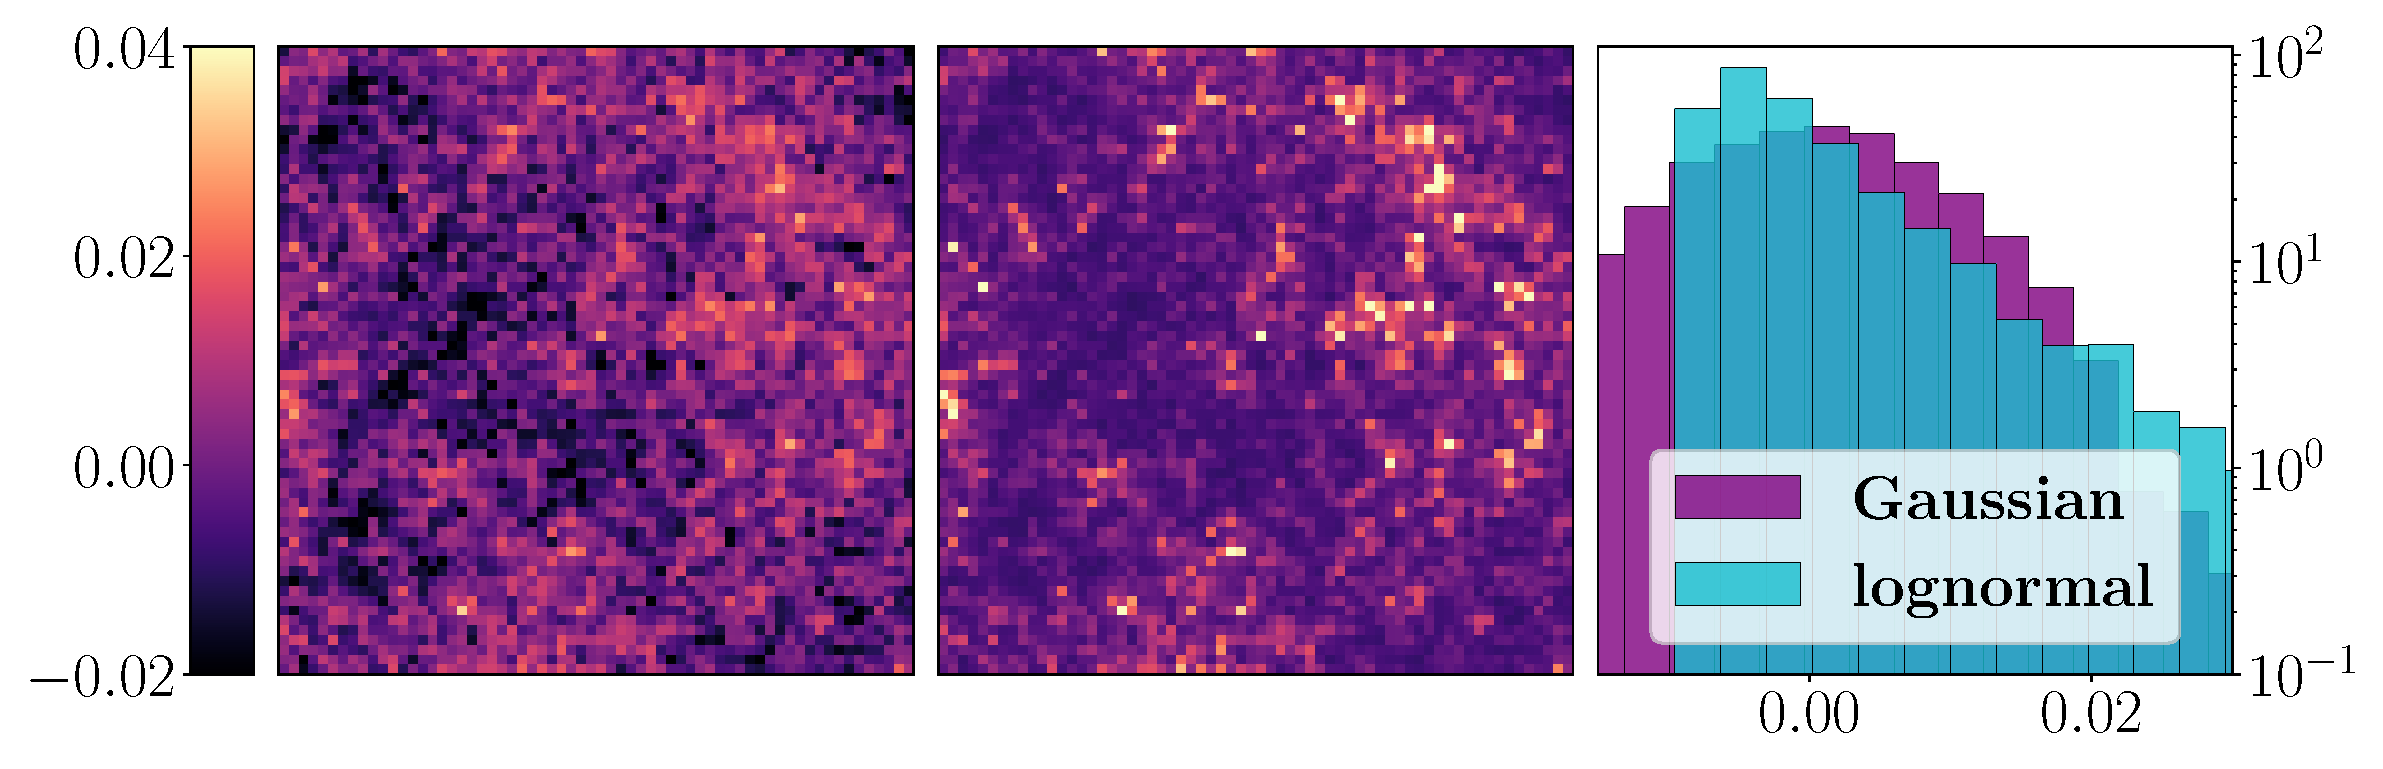
\includegraphics[width=1\textwidth]{images/4_Gaussian_lognormal_dist.pdf}
    \caption{\label{fig:fields dist} Comparison of a Gaussian map, on the left, with a lognormal map on the right. Both maps arise from the same random seed. The colorbar has been adjusted to enhance the differences between the two. The histogram plot shows the clear difference in the map distributions.}
\end{figure}

We show example realisations of the two fields in \textit{Fig. }\ref{fig:fields dist}, Gaussian on left and lognormal on the right. There's a visible difference between the two, as it can be seen clearly from the distribution plot. The main check to perform is for testing whether the generated fields recover the theoretical power spectrum. \textit{Fig. }\ref{fig:check fields} shows that this is the case for the Gaussian fields. They recover the fiducial $C(l)$ within a few percent error, with larger deviations $\sim 5\%$ at the low and high ends of the $l$-range. Instead, lognormal fields present deviations $\gtrsim 10\%$. As the lognormal transformations we use have been reported by different sources \cite{fwdmodel}\cite{lognormal}, the issue must lie with our \code{JAX} implementation of the Hankel transformation. Resolving such issues could be achieved by future iterations of this work. In this work, we restrict ourselves to the use of Gaussian fields, as it is enough to prove our thesis and show that Gaussian processes can be applied to cosmological fields.
\begin{figure}[h]
    \centering
    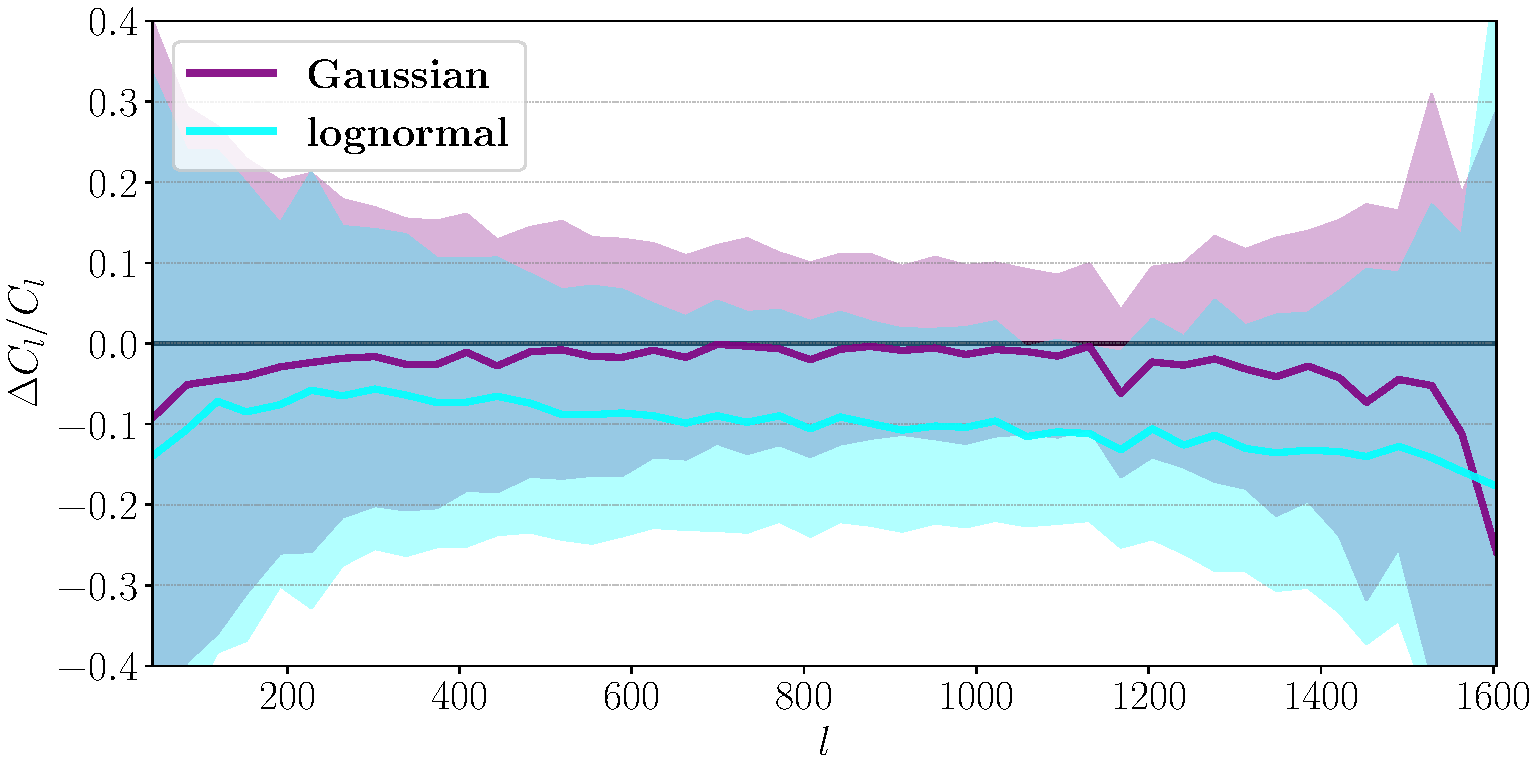
\includegraphics[width=1\textwidth]{images/4_Gaussian_lognormal_check.pdf}
    \caption{\label{fig:check fields} Power spectrum estimation from  Gaussian and lognormal maps. Mean and standard deviation are calculated with 500 realisation of both fields.}
\end{figure}

\subsection{Gaussian process priors}
\label{sec:gaussian process priors}
First, we test the ability of the kernels we have built in \textit{Sec. }\ref{sec:gaussian process kernel} to recover the power spectrum of our cosmology.  
\begin{figure}[h]
    \centering
    %\textit{Kernels comaprison}}\par
    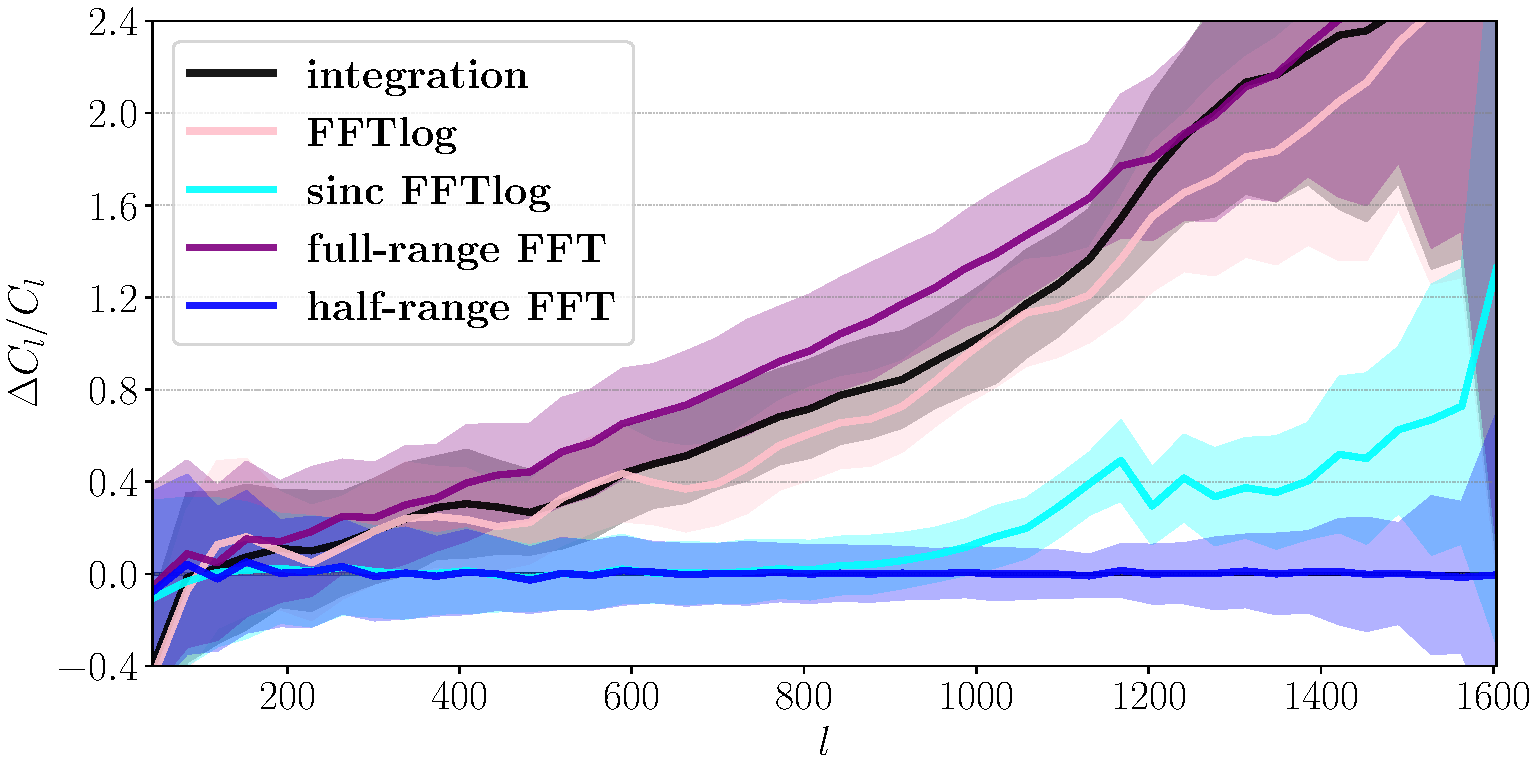
\includegraphics[width=\textwidth]{images/3_kernel_comparison.pdf}
    \caption{\label{fig:check methods} Reconstructed power spectrum from prior sample of GP with the four proposed kernels: integration, FFTlog, full-range FFT, half-range FFT and sinc FFTlog. Mean and standard deviation are calculated with 500 prior samples from each GP. }
\end{figure}
We test five models in \textit{Fig. }\ref{fig:check methods}: integration, FFTlog, full-range FFT, half-range FFT and sinc FFTlog. The first four methods are described in the Gaussian process kernels \textit{Sec. }\ref{sec:gaussian process kernel}, whereas the sinc FFTlog referes to a FFTlog model on which we applied smoothing, by multiplying the power spectrum by a factor of $sinc^4(l\frac{L}{2\pi N})$. The recovered power spectra are plotted against the fiducial power spectrum, or smoothed power spectrum for the sinc FFTlog. Mean and standard deviation associated to the plots are calculated from 500 samples. As expected the integration, FFTlog and full-range FFT perform similarly, as they all contain the same ammount of information. As these models deviate so strongly from the fiducial power spectrum we tried applying smoothing, which helps to recover half of the $l$-range at large scales. The only method that seems to be consistently recovering the fiducial power spectrum is the half-range FFT. One could argue that due to the inherent discreteness and boundedness of the fields we are working with, using FFTs is the most natural choice; also, half-range FFT uses the only grid that recovers a correlation function of the same shape as the field without having to perform binning.
\begin{figure}[h]
    \centering
    %\textit{Cosmology invariance}}\par
    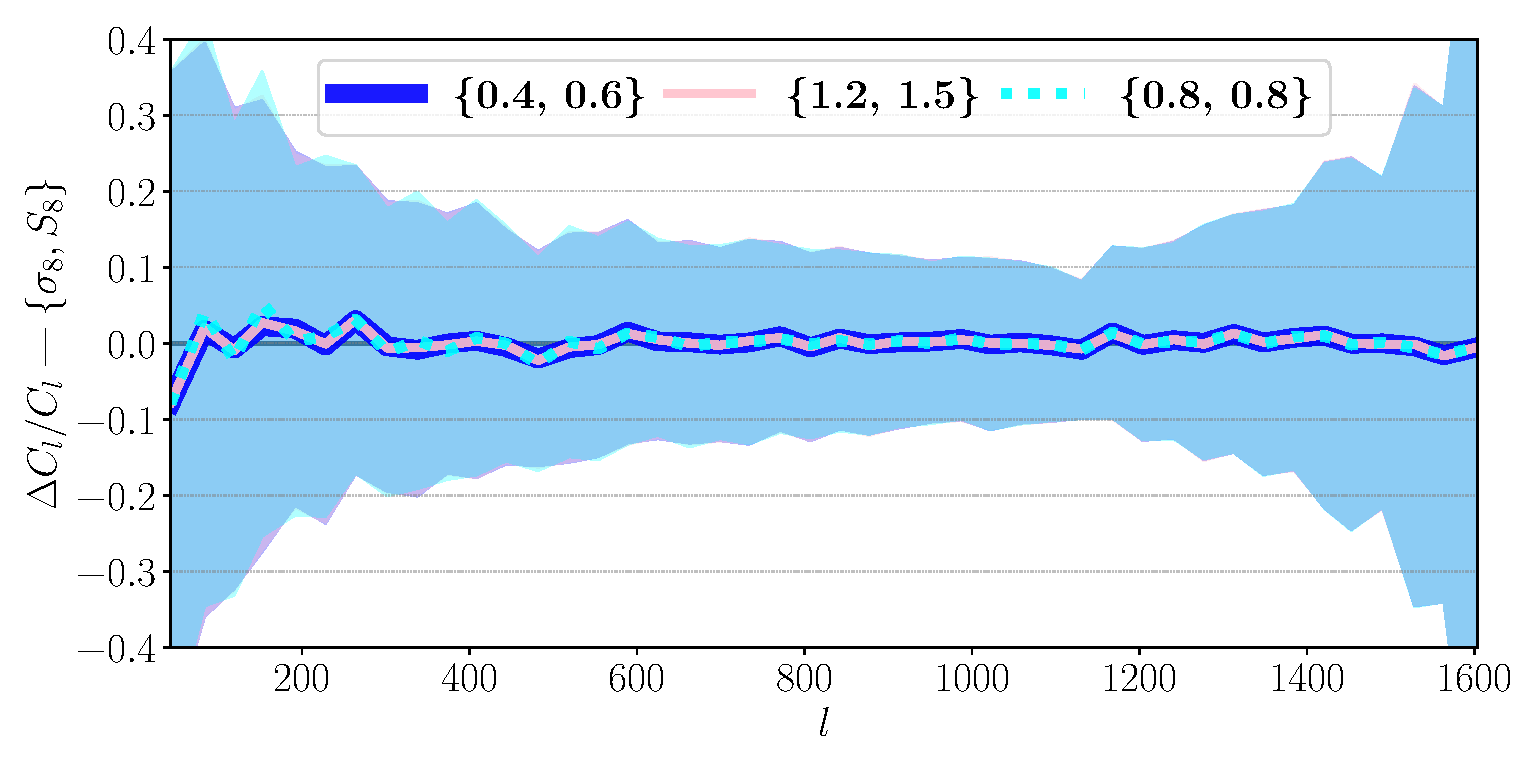
\includegraphics[width=\textwidth]{images/3_cosmology_comparison.pdf}
    \caption{\label{fig:check cosmology} Reconstructed power spectrum from prior samples of a GP, as a function of $\{\sigma_8, S_8\}$. Mean and standard deviation are calculated with 500 prior samples for each different cosmology.}
\end{figure}

We have also tested the efficacy of the half-range FFT model for different cosmologies of values $\{\sigma_8, S_8\}$ equal to $\{0.4,0.2\}$, $\{1.2,1.5\}$ and, our fiducial cosmology, $\{0.8,0.8\}$. As \textit{Fig. }\ref{fig:check cosmology} shows, the model is independent of the choice of cosmology. From here on the results will be presented assuming a kernel built with the half-range FFT model.

\section{Gaussian process map reconstruction}
\label{sec:gaussian process map reconstruction}
Armed with a reliable kernel, let's embark upon the journey of reconstructing a heavily masked cosmological field. What we will do is: create a noiseless GRF in the fiducial cosmology \textit{Tab. }\ref{tab:fiducial_cosmology}, \textit{True} map; apply a mask to obtain the \textit{Data} map; condition a Gaussian process which assumes the fiducial cosmology. \textit{Fig. }\ref{fig:GP reconstruction summary} lists the result of this operation, showing the resulting mean $\mu$ and standard deviation $\sigma$ of the conditioned GP. We also plot the ratio between residuals $\Delta=\mu-$\textit{True} and standard deviation squared, to test the goodness of fit of our model, the values of the map sum up to $\chi^2 \sim 2495$. With the mask covering $\nu=2353$ pixels, we obtain $\chi^2 / \nu = 1.06$. Of course, this is just a noiseless application, which is unreasonable for a real application.
\begin{figure}[h]
    \centering
    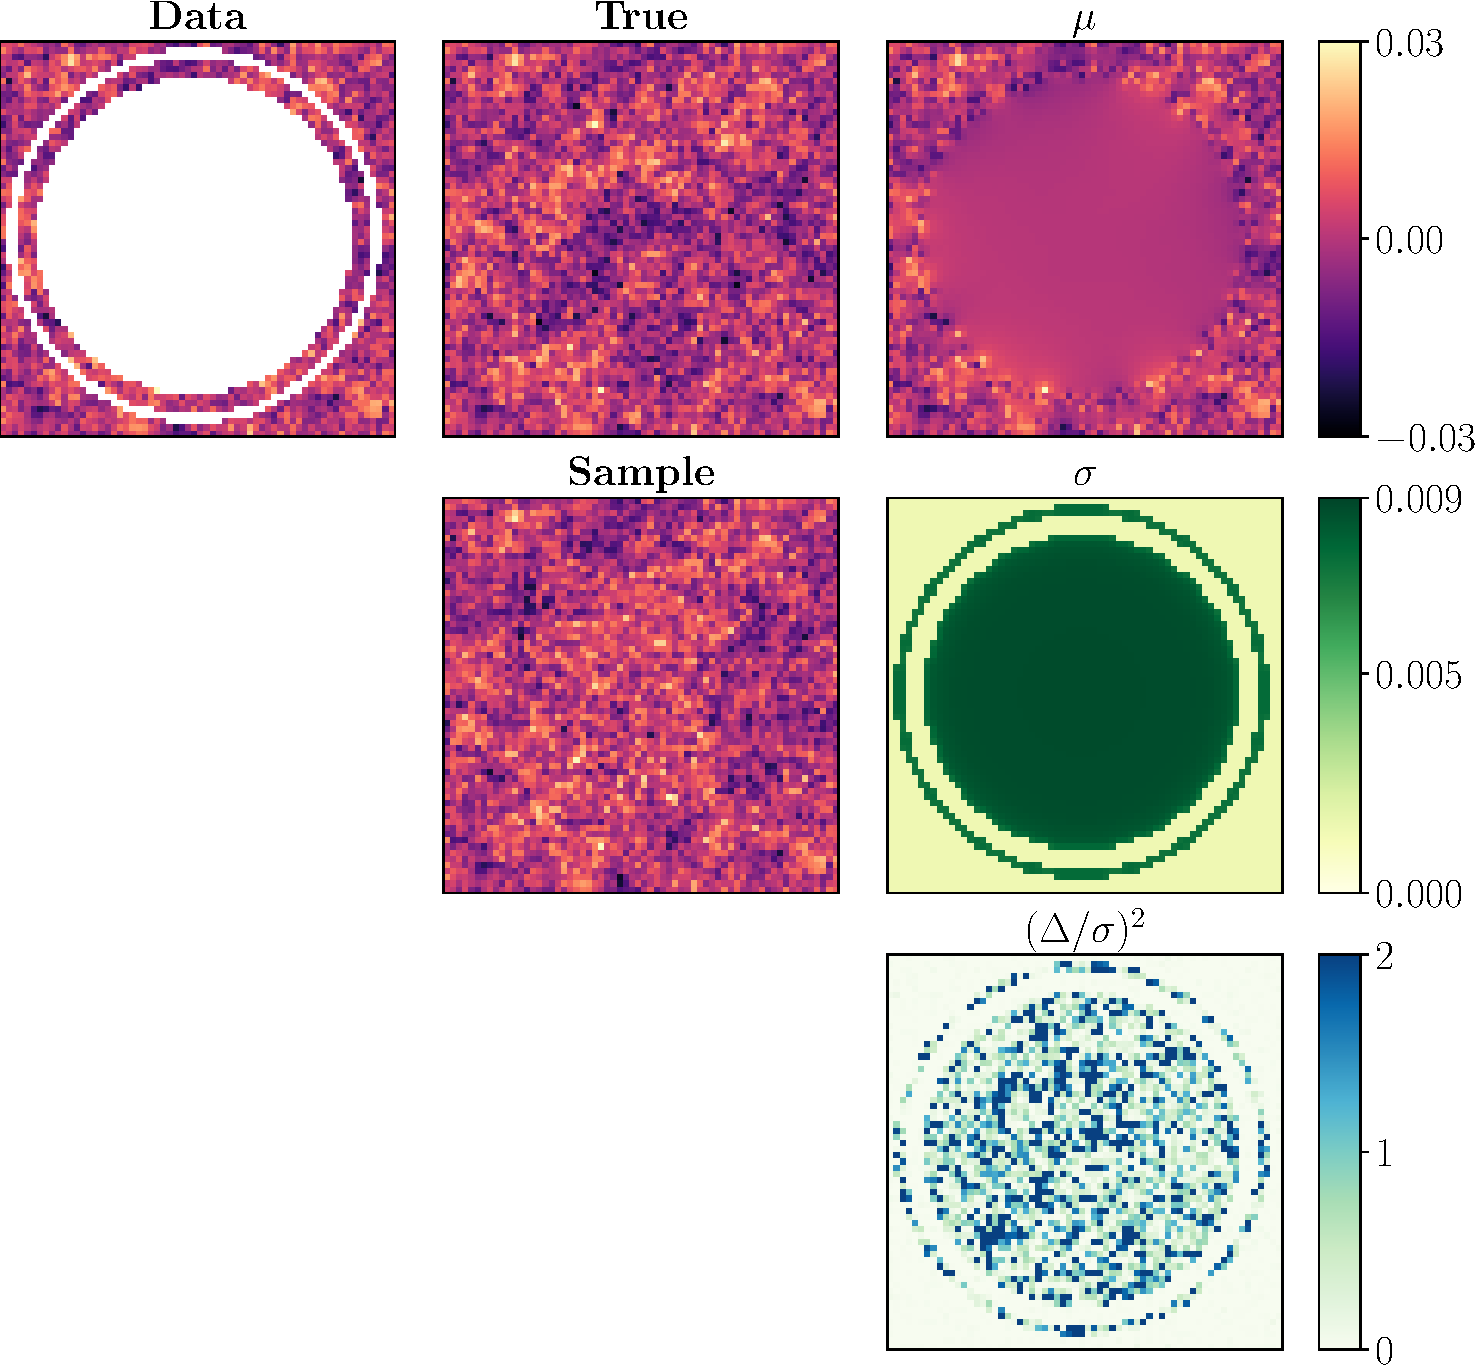
\includegraphics[width=\textwidth]{images/2_summary.pdf}
    \caption{\label{fig:GP reconstruction summary}Summary of field reconstruction abilities of a Gaussian process conditioned on data. The left column shows the masked GRF, which is our data. The middle column shows the true GRF without masks and a posterior sample drawn from the conditioned GP. The right column shows maps of the mean, standard deviation and residuals over standard deviation squared of the conditioned GP. Regions of higher uncertainty correspond to the masked regions. The residuals over standard deviation map also shows how regions with low mask recover the data.}
\end{figure}

\section{Inference of cosmological parameters}
\label{sec:inference of cosmological parameters}
To test the ability of Gaussian processes to recover cosmological parameters without any prior knowledge except a noisy and masked map, we perform a MCMC simulation to infer the posterior distributions of $\sigma_8$ and $S_8$. We use the convention 
\begin{equation}
    S_8 = \sigma_8 \sqrt{\frac{\Omega_m}{0.3}},
    \label{eq:S8}
\end{equation}
\begin{wraptable}{l}{3.7cm}
\centering
\caption{Priors used by our \code{numpyro} model for cosmological parameter inference}\label{tab:priors}
\begin{tabular}{ll}
    \toprule
     & Prior \\
    \midrule
    $S_8$ & $\mathcal{U}[0.565,1.78]$ \\
    $\sigma_8$ & $\mathcal{U}[0.4,1]$ \\
    $\Omega_m$ & $\mathcal{U}[0.15,0.95]$ \\
    \bottomrule
\end{tabular}
\end{wraptable} 
to infer deterministically a posterior for $\Omega_m$. Such a reparametrisation is needed due to the strong degeneracy between $\sigma_8$ and $\Omega_m$. \textit{Eq. }\eqref{eq:S8} breaks this degeneracy, changing the geometry of the sampling space and making the sampling more consistent. The model assumes uninformed flat priors for the cosmological parameters, as shown in \textit{Tab. }\ref{tab:priors}, such prior bounds are also in accordance with the \code{jaxcosmo} release \cite{jaxcosmo}. The likelihood of the model is given by a Gaussian process distribution conditioned on \textit{Data}, with a standard deviation equal to the noise applied to the map. The analysis is coded with \code{numpyro} \cite{numpyro} \cite{numpyro2}, using a the \textit{No-U-Turn Sampler (NUTS)} method with \code{max_tree_depth=16}, \code{target_accept_prob=0.8}. We simulate 8 chains for the $32\times32$ grid and 4 chains for the $64\times64$. Each chain performs 1000 warmup steps and 3000 samples. 


\subsection{One parameter}
As a first step and for a consistency check, we run the inference model for one cosmological parameter, keeping all others fixed. Using a $64\times64$ grid with $n_g=10 \text{ galaxies}/\text{arcmin}^2$. In \textit{Fig. }\ref{fig:MCMC one parameter} we show the inferred distribution for both $\sigma_8$ and $\Omega_m$. We find that we are able to recover the true value for both parameters within two sigmas, $\sigma_8 = 0.776\pm0.015$ and $\Omega_m = 0.284\pm0.010$. We notice a slight tendency of the inferred distribution to be biased low; a tendency we also observe next for both sampled parameters, $S_8$ and $\sigma_8$.
\begin{figure}[h]
    \begin{minipage}[b]{0.48\textwidth}
        \centering
        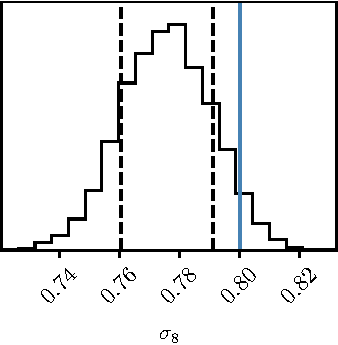
\includegraphics[width=\textwidth]{images/6_MCMC_sigma_parameters.pdf}
    \end{minipage}
    \hfill % Add horizontal space between minipages
    \begin{minipage}[b]{0.48\textwidth}
        \centering
        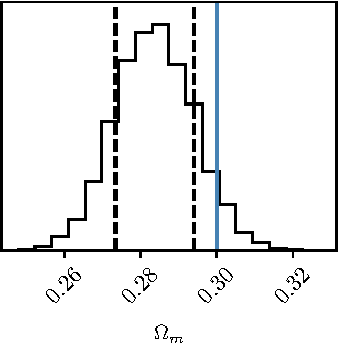
\includegraphics[width=\textwidth]{images/6_MCMC_omega_parameters.pdf}
    \end{minipage}
\caption{\label{fig:MCMC one parameter} Inferred posterior distribution of $\sigma_8$ on the left and $\Omega_m$ on the right. Dotted lines indicate the $1\sigma$ level. Truth values corresponding to the fiducial cosmology are indicated in blue.}
\end{figure}

\subsection{Two parameters}
\subsubsection{Effect of noise}
\begin{table}[h]
\centering
\caption{List of inferred cosmological parameters inferred by the model with a small $32\times32$ grid and for a fixed true GRF realisation. We present the cosmological parameters inferred as we increase the noise level, corresponding to $n_g = 4$, $10$, $30$ and $100 \text{ galaxies}/\text{arcmin}^2$.}\label{tab:inferred cosmological parameters}
\begin{tabular}{lcccc}
    \toprule
    $\sigma_\text{noise}$ & $0.0069$ & $0.0044$ & $0.0025$ & $0.0014$\\
    \midrule
    $S_8$      & $0.716\pm0.043$ & $0.733\pm0.040$ & $0.747\pm0.041$ & $0.752\pm0.042$\\
    $\sigma_8$ & $0.645\pm0.157$ & $0.628\pm0.158$ & $0.632\pm0.166$ & $0.631\pm0.170$\\
    $\Omega_m$ & $0.423\pm0.164$ & $0.469\pm0.175$ & $0.485\pm0.186$ & $0.497\pm0.193$\\
    \bottomrule
\end{tabular}
\end{table}
We perform some tests on low resolution $32\times32$ grids to see the effect that the noise level has on the recovered parameters, see \textit{Tab. }\ref{tab:inferred cosmological parameters}. Here we report the inferred cosmological parameters for one data realisation and different noise levels, corresponding respectively to $n_g = 4$, $10$, $30$ and $100 \text{ galaxies}/\text{arcmin}^2$, see \textit{Eq. }\eqref{eq:noise}. The inferred value of $S_8$ can vary as much as a full $\sigma$ between high and low noise runs. Keeping in mind that $\sigma_8$ and $\Omega_m$ are extremely unreliable due to relative uncertainties of $\sim 25-30\%$ caused by the degeneracy: as a general trend we notice $\Omega_m$ gets bigger when $\sigma_8$ gets smaller with less noise.

\subsubsection{Inferred cosmological parameters}
Running the model for a larger $64\times64$ grid with $n_g=10 \text{ galaxies}/\text{arcmin}^2$, gives much better constraints on the cosmological parameters. We present the values recovered by the posterior distributions, listed as follows in \textit{Tab. }\ref{tab:inferred cosmological parameters (64,64)}. 
\begin{table}[h]
    \centering
    \caption{\label{tab:inferred cosmological parameters (64,64)} Mean and sigma values recovered from the inferred distributions of the cosmological parameters.}
    \begin{tabular}{ccc}
        \toprule
        $S_8$ & $\sigma_8$ & $\Omega_m$\\
        \midrule
        $0.762\pm0.028$ & $0.745\pm0.151$ & $0.353\pm0.143$\\
        \bottomrule
    \end{tabular}
\end{table} 

\textit{Fig. }\ref{fig:MCMC two parameters} shows the inferred posterior distributions and contours for the three cosmological parameters $\sigma_8$, $\Omega_m$ and $S_8$. Looking at the contours, we obtain the well known banana-shaped degeneracy between $\sigma_8$ and $\Omega_m$. The $S_8$ and $\Omega_m$ contour presents sharp cuts for  high and low $\Omega_m$, indicating an issue with the bounds of the uniform priors imposed. Unfortunately the \code{jaxcosmo} package does not allow for the choice of priors to be wider than what shown in \textit{Tab. }\ref{tab:priors}, as the model then starts to have divergent samples.
\begin{figure}[h]
    \centering
    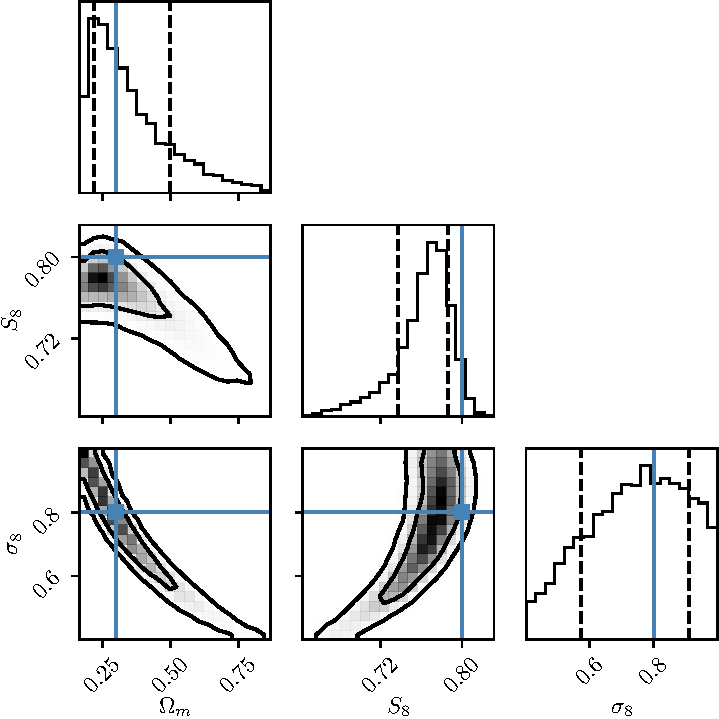
\includegraphics[width=\textwidth]{images/5_MCMC_two_parameters.pdf}
    \caption{\label{fig:MCMC two parameters} Inferred posterior distributions of $S_8$, $\sigma_8$ and $\Omega_m$. For noise level $\sigma_\text{noise}\sim 0.0088$. Contours indicate the $1\sigma$ and $2\sigma$ credible interval respectively. Dotted lines indicate the $1\sigma$ level. Truth values corresponding to the fiducial cosmology are indicated in blue.}
\end{figure}

\subsection{Posterior checks}
Following the two parameter inference model, we perform some posterior checks at the map level \cite{fwdmodel2}. \textit{Fig. }\ref{fig:MCMC summary}
sums up the ability of the model to recover the true map, noiseless and unmasked. Here we present the run with noise level $\sigma_\text{noise}\sim 0.0088$ and a $64\times64$ grid. We show the mean and standard deviation for the sample with highest likelihood out of the $12000$. The mean field $\mu$ is visibly different to the true field in the masked regions and it seems to be of overall lower amplitude. The sample map is comparable to the noisy data; which is to be expected, as the internal noise given to the Gaussian process is the same as the noise level of the data. The standard deviation map $\sigma$ presents an overall amplitude comparable to the noise level $\sim 0.010$, with higher values for the masked regions. Summing up the map values of the residuals divided by standard deviation squared, we obtain a $\chi^2\sim 1297.4$. Compared to the number of free parameters $\nu$ in our inference model, which for a $10\%$ mask and a $64\times64$ grid, is $\nu=3689$. The value of $\chi^2$ therefore seems to be low, indicating that the noise level assumed by the GP is overestimated. This is supported by the fact that the sample map looks just as noisy as the data, according to \textit{Fig. }\ref{fig:residuals vs noise}, its distribution is in fact just as wide as the noise.

\begin{figure}[h]
    \centering
    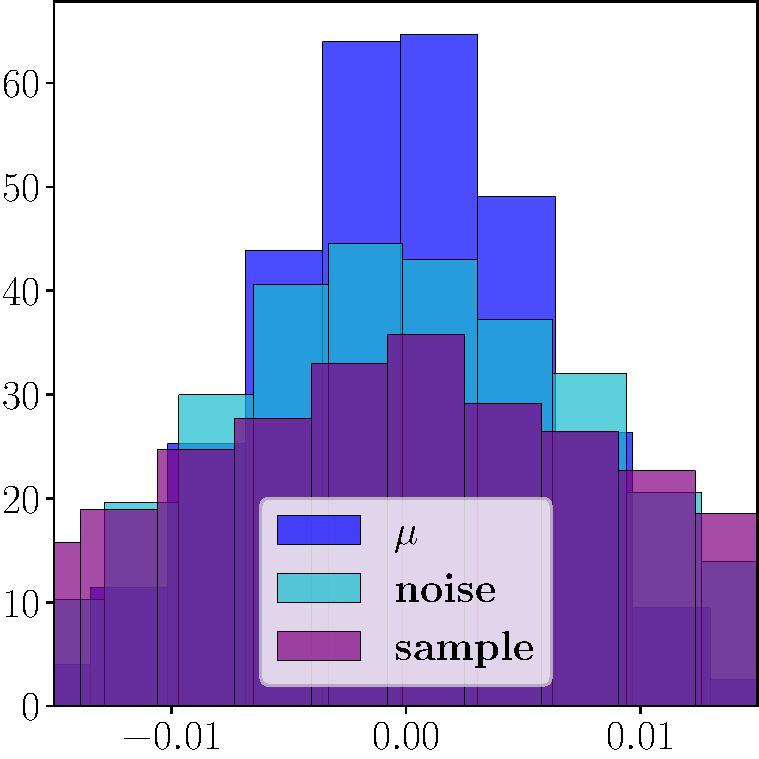
\includegraphics[width=0.5\textwidth]{images/5_residuals_vs_noise.pdf}
    \par \hspace{0.3cm} \textit{Residuals}
    \caption{\label{fig:residuals vs noise} Residual distributions of the mean and sample compared to noise. The mean is less spread, whereas the sample is wider.}
\end{figure}

\begin{figure}[h]
    \centering
    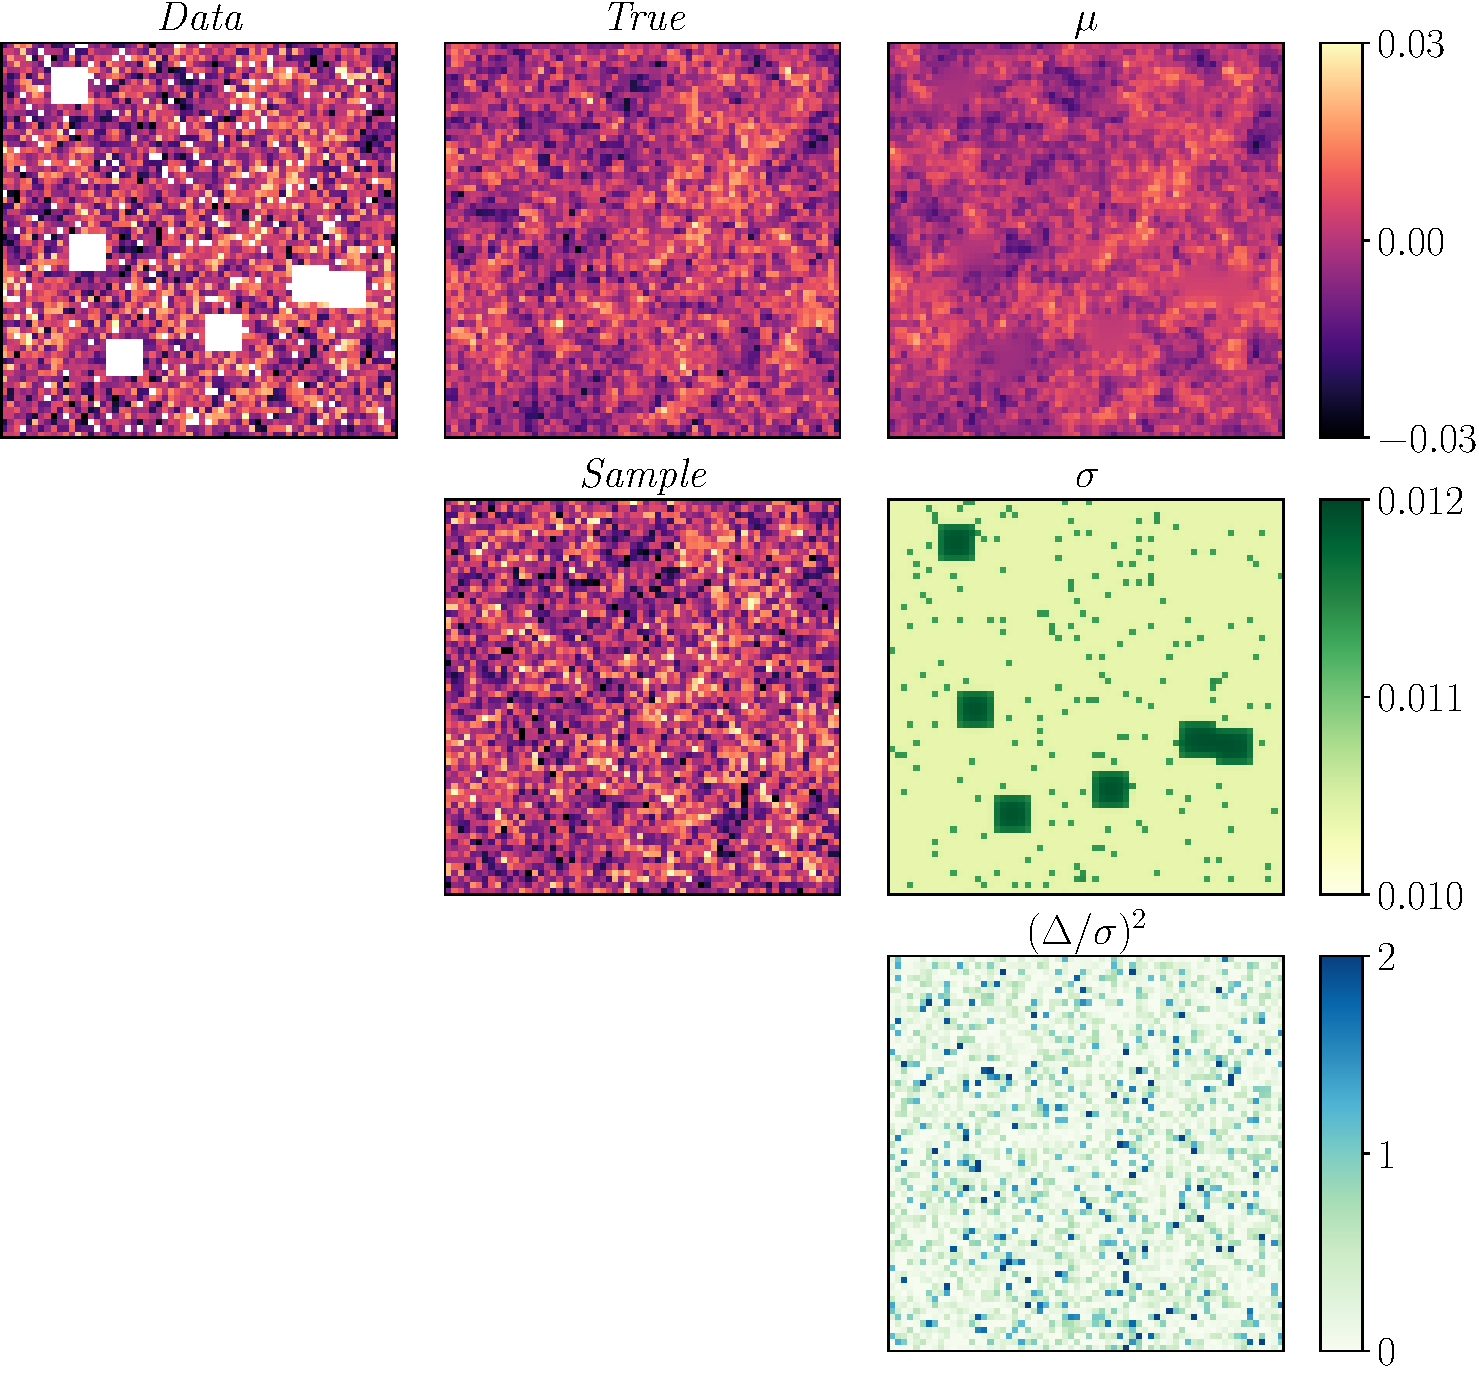
\includegraphics[width=\textwidth]{images/5_summary.pdf}
    \caption{\label{fig:MCMC summary} Summary of the two parameter inference at the map level. The left column shows the masked and noisy GRF realisation used, which is our data. The middle column shows the true GRF and a sample from the conditioned GP. The right column shows maps of the mean, standard deviation and residuals over standard deviation squared resulting from the numpyro model sample with highest likelihood. Regions of higher uncertainty correspond to the masked regions.}
\end{figure}